\documentclass[12pt]{article}
\usepackage{pgf, tikz}
\usepackage{amsmath, amsfonts, amssymb, graphicx}
\usepackage{float}
\usepackage{subfig}
\usepackage[utf8]{inputenc}
\usepackage[spanish]{babel}
\usepackage{amsthm}
\usepackage{caption}

\setlength{\textheight}{23cm} \setlength{\evensidemargin}{0cm}
\setlength{\oddsidemargin}{-.5cm} \setlength{\topmargin}{-3cm}
\setlength{\textwidth}{17.5cm} \setlength{\parskip}{.2cm}


%opening

\begin{document}
	\begin{picture}(80, 80)
	\put(170,0){\hbox{
\includegraphics[scale=0.6]{cimat_logo.png}}}
	\end{picture}
	
	\begin{center}
		\begin{huge}
			Centro de Investigación en Matemáticas, A.C.
		\end{huge}
	\end{center}

	\begin{center}
		\begin{large}
			Descripción tarea 1 - Optimización
		\end{large}
	\end{center}
	
	\begin{center}
		\textbf{Erick Salvador Alvarez Valencia}
	\end{center}

	\begin{center}
		29 de Enero de 2018
	\end{center}



%\maketitle

%\tableofcontents

\section{Introducción}
En el presente reporte se describirán los resultados obtenidos para la tarea 1. En dicha tarea se tiene que hacer principalmente la implementación de la factorización de Cholesky así como demostrar que con ella podemos ver si una matriz es simétrica y definida positiva. Al final de este reporte se mostrarán los resultados de las ejecuciones para diferentes casos de matrices.

\section{Matriz simétrica y definida positiva y factorización de Cholesky}

\subsection{Descripción}
Lo primero que se tiene que hacer es hacer la función que calcule la factorización de Cholesky. La cual la definimos de la siguiente forma:\\

Sea $A$ una matríz simétrica y definida positiva, ahora la factorización de Cholesky es una matriz $L$ que cumple: $A = LL^T$.\\

Una vez que tenemos dicha factorización podemos empezar a seguir el procedimiento descrito en la tarea, en donde primeramente verificamos si la matriz $A$ es simétrica, para ello comprobamos que $||A - A^T|| < \epsilon$ y para lo cual usamos una norma natural como la norma 1.\\
En caso de que $A$ no sea simétrica la sustituimos por $\frac{A + A^T}{2}$ en donde dicha matriz si es simétrica.\\
Ahora intentamos calcular la factorización de Cholesky de la matriz anterior, si no se puede calcular esta factorización entonces la matriz no es definida positiva y por lo tanto hay que hacerle una perturbación de la siguiente forma:

$$A^* = A + \lambda I$$

Donde $\lambda > 0$.\\
Esto se hace una y otra vez hasta que se pueda realizar la factorización de Cholesky. A continuación se demostrará el porqué dicha perturbación funciona.\\

Ya se dijo que $\lambda > 0$ ahora sabemos que la matriz $A$ es simétrica ya que para este punto lo hemos comprobado o de otra forma, provocado.\\
Lo siguiente es ver la definición de una matriz definida positiva.\\

Una matriz $A$ es definida positiva si para todo vector $x \neq 0$ se tiene que

\begin{align}
\label{eqn:eqlabel}
\begin{split}
x^T A x > 0
\end{split}
\end{align}

Ahora teniendo en cuenta de que $A$ es una matriz perturbada en sus diagonales, tal que $A = B + \lambda I$ cambiamos esto anterior en (1) obteniendo.

\begin{align}
\label{eqn:eqlabel}
\begin{split}
x^T (B + \lambda I) x > 0
\end{split}
\end{align}

Ahora desarrollamos lo anterior

\begin{align}
\label{eqn:eqlabel}
\begin{split}
x^T B x + \lambda x^T I x > 0
\end{split}
\end{align}

Ahora, tenemos que el primer término de la suma anterior cumple con la definición de una matriz definida positiva y de la misma forma dicho término forma un escalar. Por otra parte y analizando el segundo término podemos ver que tenemos un producto punto con el mismo vector $<x, x>$ lo cual es igual a la norma de dicho vector al cuadrado $||x||^2_2$ y, por definición sabemos que $\lambda > 0$ entonces todo ese término resultará siempre positivo.\\
Entonces lo que se puede ver es que en caso de que $x^T B x \leq 0$, el término de la derecha puede provocar que al final sea positivo siempre y cuando elijamos el $\lambda$ adecuado, y por lo mismo vamos aumentándolo poco a poco ya que no queremos que la matriz se perturbe demasiado.

\section{Ejemplo de ejecución}
A continuación se mostrará el resultado de la ejecución del programa usando tres tipos de matrices.

\begin{figure}[H]
	\centering
	\subfloat[][Figura 1. Ejecución del programa con una matriz simétrica y definida positiva.]{
		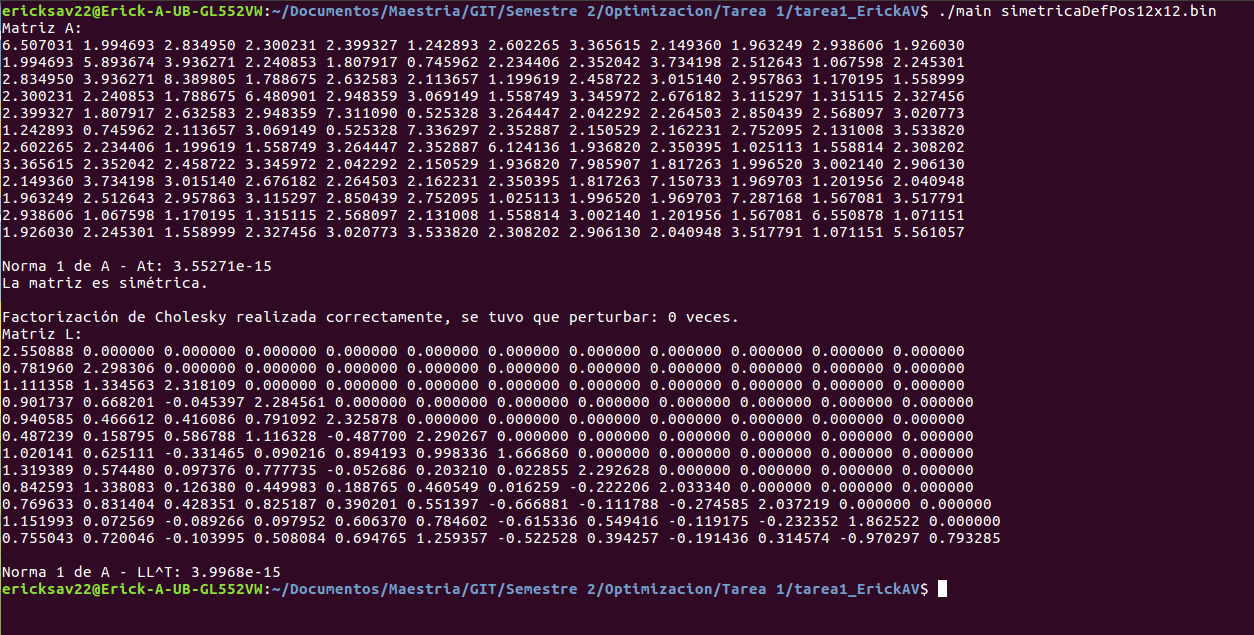
\includegraphics[scale=0.4]{SimetricaDefPos.png}
	}\hfill
\end{figure}

En la Figura 1 podemos ver que se verifica que la matriz A es primeramente simétrica, donde la norma $||A - A^T||$ es de orden $e^{-15}$. Posteriormente vemos que la matriz es definida positiva ya que se pudo factorizar sin ninguna perturbación.

\begin{figure}[H]
	\centering
	\subfloat[][Figura 2.1. Ejecución del programa con una matriz simétrica y  no definida positiva.]{
		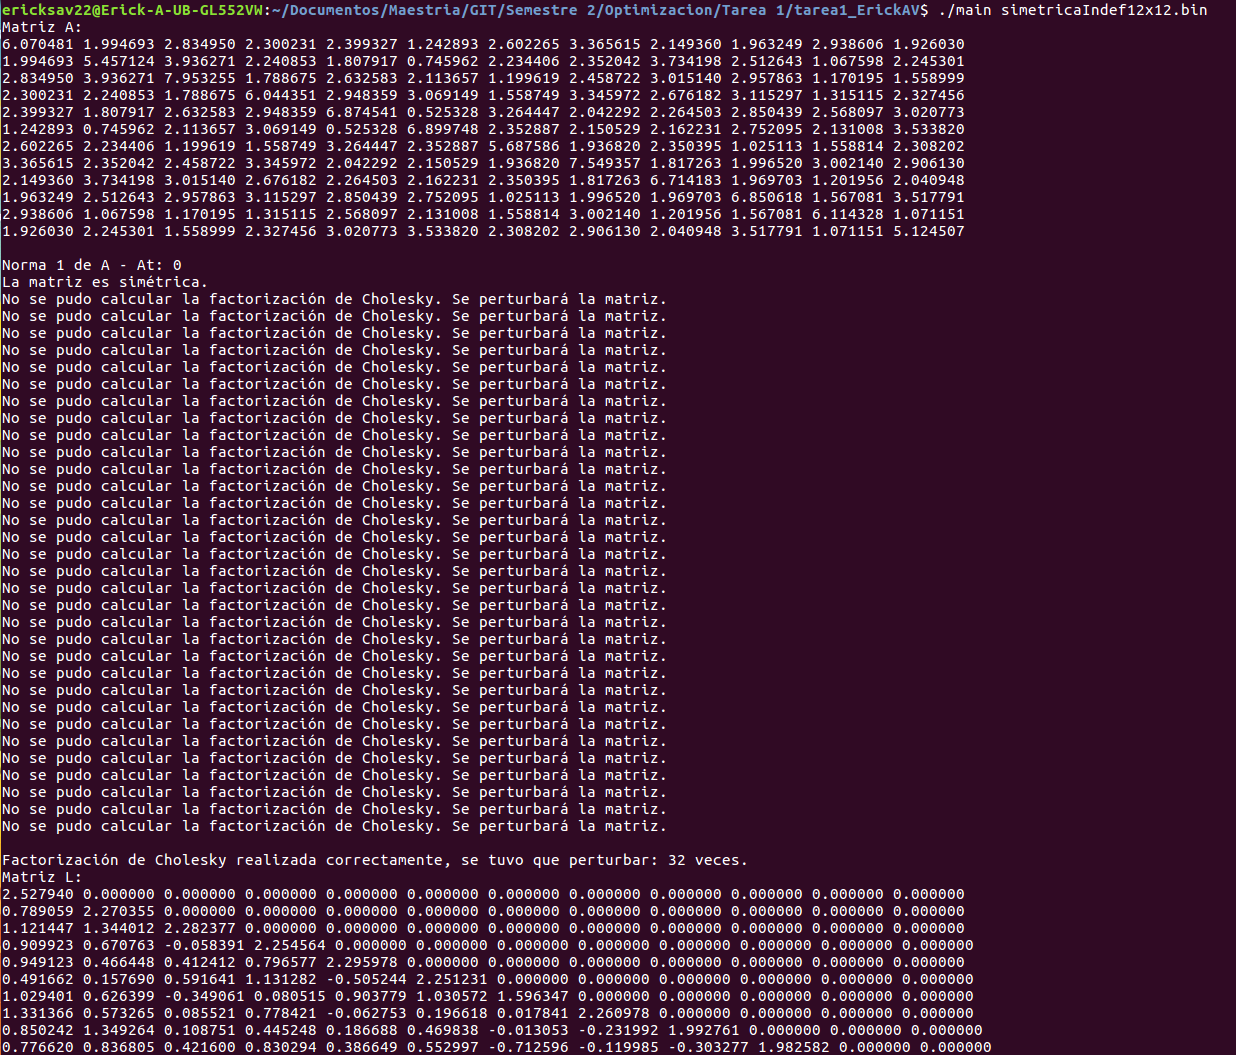
\includegraphics[scale=0.4]{SimetricaNoDefPos1.png}
	}\hfill
\end{figure}

\begin{figure}[H]
	\centering
	\subfloat[][Figura 2.2. Ejecución del programa con una matriz simétrica y  no definida positiva.]{
		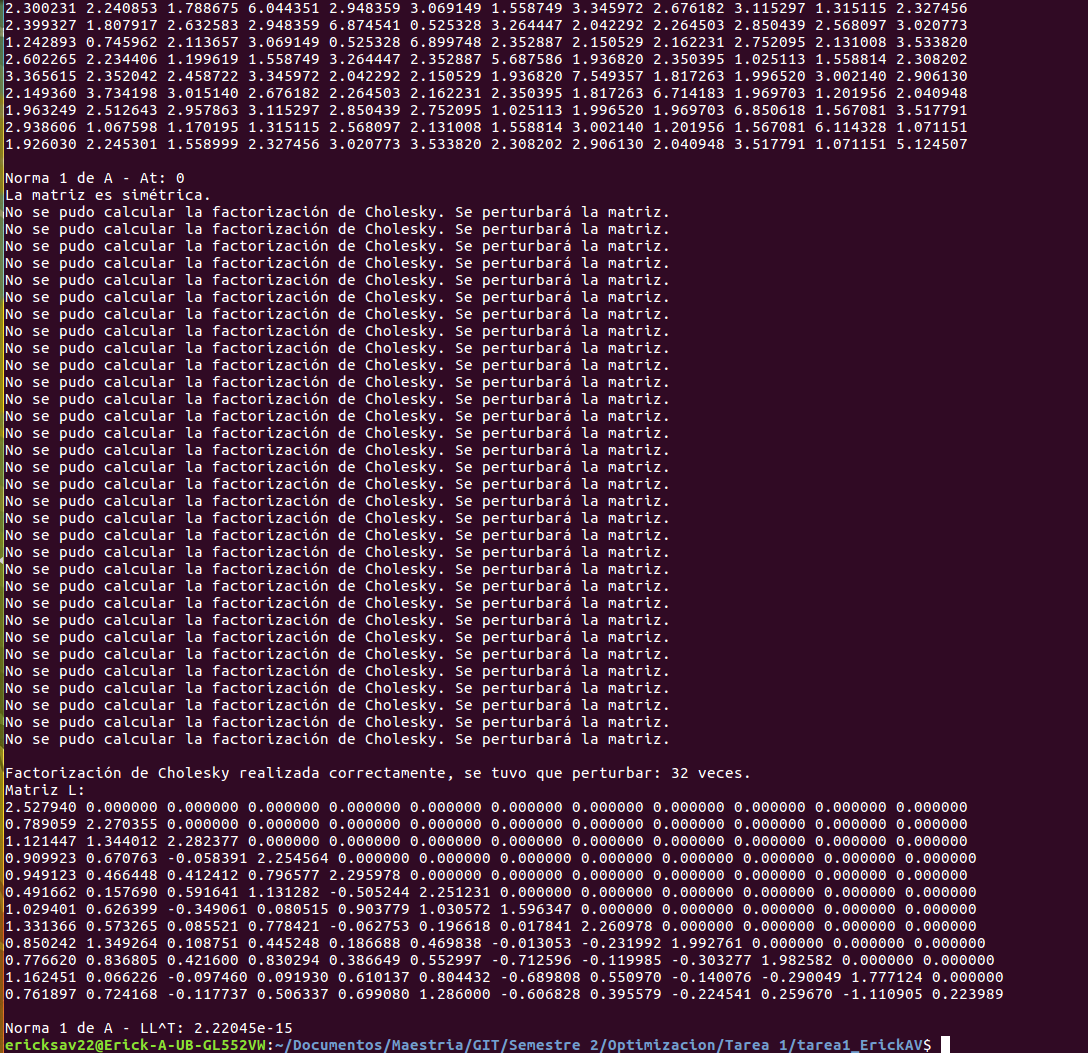
\includegraphics[scale=0.4]{SimetricaNoDefPos2.png}
	}\hfill
\end{figure}

Al igual que en el caso anterior, se puede ver que la matriz $A$ es simétrica, mas aún no es definida positiva y esto se ve reflejado en que hay que perturbarla 32 veces para lograr su factorización de Cholesky.

\begin{figure}[H]
	\centering
	\subfloat[][Figura 3. Ejecución del programa con una matriz no simétrica y  no definida positiva.]{
		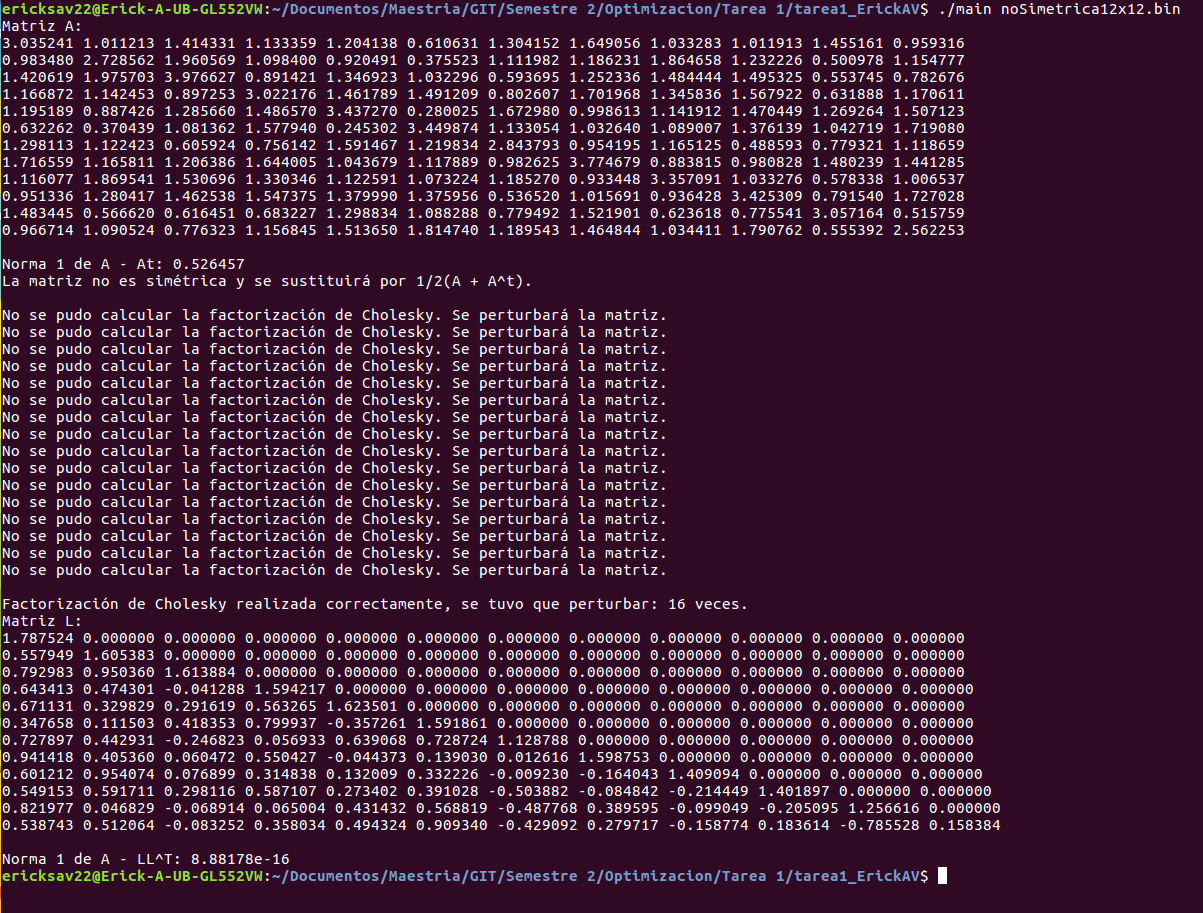
\includegraphics[scale=0.4]{NoSimetrica.png}
	}\hfill
\end{figure}

En este último caso se puede apreciar por la norma de $A - A^T$ que la matriz no es simétrica, por lo cual se sustituye por una que si lo es. Y por último vemos que tampoco es definida positiva ya que se tuvo que perturbar 16 veces para lograr su factorización de Cholesky.

\section{Compilación y ejecución}
\textbf{Para compilar:} En la carpeta encontraremos los archivos $.c$ y $.h$ con los que se podrá compilar el ejecutable. De la misma forma, en conjunto con los archivos anteriores, también podremos encontrar un Makefile para, en caso de encontrarse en linux, compilar de manera sencilla.

\begin{enumerate}
	\item \textbf{Compilar usando Makefile:} En la terminal, nos colocamos en el directorio donde se encuentre el programa, y ejecutamos el comando $make$, automáticamente se realizará la compilación y se generará el ejecutable. El Makefile también contiene el comando $make\ help$ el cual mostrará todas las opciones disponibles.
	\item \textbf{Compilar directamente:} De la misma forma, podemos compilar directamente usando los siguientes comandos (en terminal):
	\begin{itemize}
		\item gcc -c main.c -o obj/main.o
		\item gcc -c memo.c -o obj/memo.o
		\item gcc -c matriz\_vector.c -o obj/matriz\_vector.o
		\item gcc -c met\_num.c -o obj/met\_num.o
		\item gcc -o main obj/main.o obj/memo.o obj/matriz\_vector.o obj/met\_num.o\ -lm
	\end{itemize}
\end{enumerate}

\textbf{Para ejecutar:} Únicamente debemos de usar el comando $./main$ para ejecutar el programa en consola, este recibe el siguiente argumento:
\begin{itemize}
	\item \textbf{Un string:} El nombre del archivo binario que contiene la matriz a ser procesada.
\end{itemize}

El programa validará que la matriz sea simétrica, de no serlo la sustituye por $\frac{A + A^T}{2}$ y posteriormente aplicará el método de Cholesky, en caso de no poderse factorizar la matríz se perturbará en la diagonal. Al final se imprimirá $||A - LL^T||_2$.\\

\textbf{Ejemplo de ejecución:} ./main simetricaDefPos12x12.bin\\

\end{document}
